\subsection{Anatomy of the remaining error}
\label{sec:anatomy}

\begin{figure}[tbp]
  \centering
  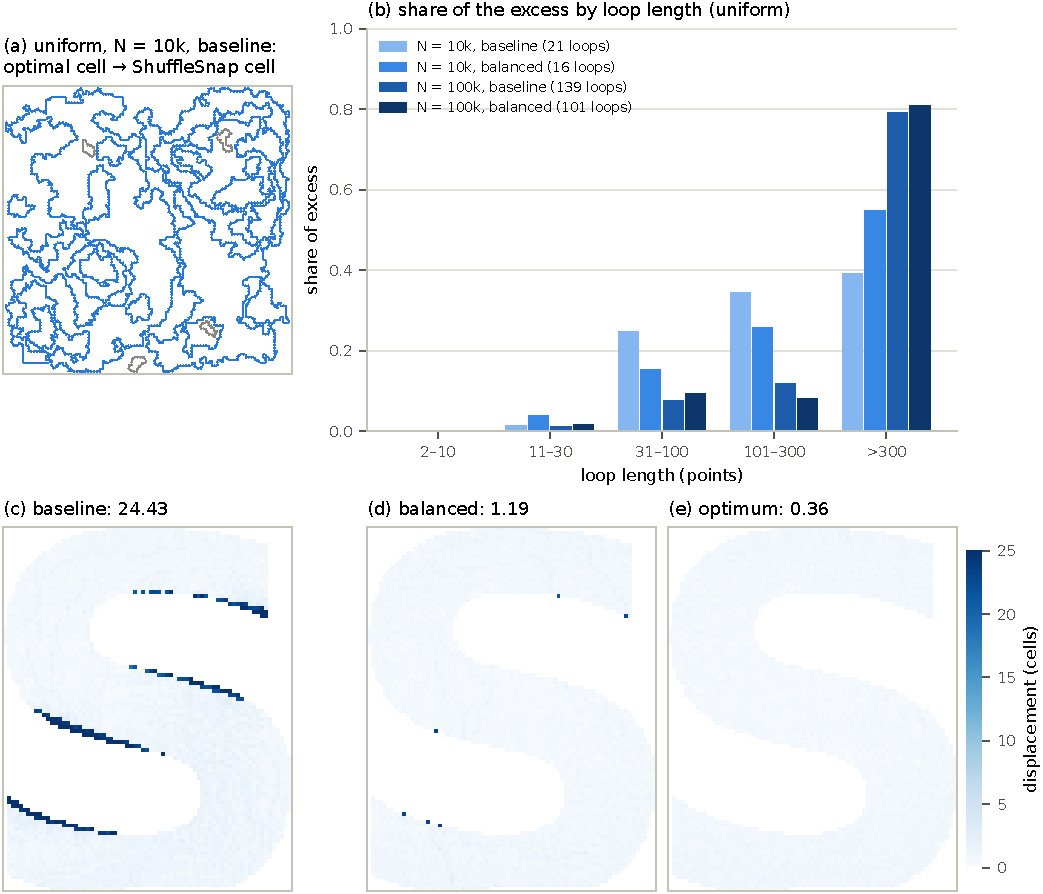
\includegraphics[width=\linewidth]{figures/fig_failures.pdf}
  \caption{Where \ShuffleSnap\ loses to the optimum (development instances, shown for
  mechanism rather than as claims). (a)~10{,}000 uniform points, default preset. Each arrow goes
  from a point's optimal cell to its \ShuffleSnap\ cell. The two layouts differ by closed
  loops of one-cell moves; loops longer than 30 points are blue. (b)~Share of the excess
  carried by loops of each length, for the fast and default presets: at $10^5$ points, about
  80\% of it sits in loops of more than 300 points. (c--e)~4{,}000 points drawn uniformly
  inside the rectilinear S-shaped mask, so that the optimum moves every point by less than a
  cell. With $6\times6$ windows and halving strides, points are routed across the concave bays
  and end up in long lines along their edges; the default preset leaves fewer such lines. Numbers are mean squared displacement.}
  \label{fig:failures}
\end{figure}

Why does a method that solves every window exactly still miss the optimum on uniform
data, by 0.84\% at $10^5$ points? Compare a \ShuffleSnap\ layout with the certified optimum. The
permutation that turns one into the other splits into cycles
(Figure~\ref{fig:failures}a). Almost all the excess sits in a handful of very long
cycles, in which every point is shifted by about one cell, so the layout is locally
rotated along a closed curve (Figure~\ref{fig:failures}b). Such a loop is invisible to
every window:
\begin{itemize}
\item Inside a stride-1 window, the part of a loop is a run of points shifted
  consistently by one cell, which is already the best arrangement of that occupant set.
  Undoing the loop requires moving one point out at one end of the run and one in at
  the other end.
\item Coarser windows cannot help either. A one-cell shift moves a point to another
  residue class, and a strided window only permutes points within one class.
\end{itemize}
Indeed, three extra cycles of stride-2 and stride-1 rounds after convergence changed
nothing on held-out uniform instances.

\paragraph{A constructed fixed point.} The argument can be checked directly. Put the
points exactly on the cell centers of a $64\times48$ grid, so that the optimum is the
identity with cost 0. Then rotate an axis-aligned ring of cells by one step: the point of
each ring cell moves to the next ring cell, so the cost equals the number $L$ of ring
cells. We ran the complete $\sqrt2$ schedule from this layout, with every stride and
every tiling, followed by stride-1 rounds to convergence. For windows of side
$w\in\{5,6,8,12,16\}$, a ring larger than the window was never touched (0 points moved), so
the result has cost $L$ against an optimum of 0. A ring of side at most $w/2+1$ always
lies inside one of the four shifted tilings and was repaired. A $6\times6$ ring
survived $6\times6$ windows when it straddled the borders of all four tilings. Relative
excess over the optimum is therefore unbounded for this method, and the package's test
suite includes this configuration as a documented limitation.

On real inputs, larger windows remove the shorter loops, and the $\sqrt2$ schedule creates
fewer loops in the first place, but the long loops remain: at $10^5$ uniform points, loops of
more than 300 points carry about 80\% of the default's excess (Figure~\ref{fig:failures}b).
Their number and total length grow with $N$, which is why the default's excess on
uniform points grows from 0.1\% at $10^3$ points to 0.84\% at $10^5$ and 1.3\% at $10^6$
(Section~\ref{sec:scaling}).

Masks make the same mechanism visible at a larger scale (Figure~\ref{fig:failures}c--e).
At a coarse stride, a window's cells can lie on both sides of a concave bay, so mass
gets routed across the bay. By the time the stride is 1, fixing the routing would
require moving a whole arm's worth of points along the arm, which no window can do.
On points drawn uniformly inside the S, where the optimum costs 0.17 cells$^2$ per point, $6\times6$
windows with halving strides ended at 32 cells$^2$ per point, with the misrouted points lined up
along the bays. The default's larger windows and finer $\sqrt2$ schedule revisit
intermediate scales and reduce the error (6.3 cells$^2$ per point) but do not remove it; the
held-out numbers are in Section~\ref{sec:masks}.

A mask can also cut exchanges off entirely. Two usable cells trade occupants only if some
scheduled window contains both. On a one-row mask whose only usable columns are 0 and 9,
stride 2 puts the two cells in different residue classes, and an 8-wide stride-1 window never
holds both. A swapped pair therefore stays swapped under the default preset, at any number of
rounds. The quality preset's 12-wide windows happen to repair this example, but not the
general problem: a mask guarantees a valid layout, not reach. The package's tests include
this case.
